\documentclass{article}
\usepackage[utf8]{inputenc}
\usepackage{hyperref}
\usepackage[letterpaper, portrait, margin=1in]{geometry}
\usepackage{enumitem}
\usepackage{amsmath}
\usepackage{booktabs}
\usepackage{graphicx}

\usepackage{hyperref}
\hypersetup{
colorlinks=true,
    linkcolor=black,
    filecolor=black,      
    urlcolor=blue,
    citecolor=black,
}
\usepackage{natbib}

\usepackage{titlesec}
  
\title{Homework 3}
\author{Ioanna Maria Spyrou}
\date{Spring semester 2021}
  
\begin{document}
  
\maketitle


1.(a) Since $y_i = e^{\alpha}\delta^{d_i}z_i^{\gamma}e^{\eta_i}$, if we take $ln$ on this relationship we get:\\
\\
$ln(y_i) = ln(e^{\alpha}\delta^{d_i}z_i^{\gamma}e^{\eta_i}) = ln(e^{\alpha} + ln\delta^{d_i} + lnz_i^{\gamma} + lne^{\eta_i} = \alpha + ln(\delta) d_i + \gamma ln(z_i) + \eta_i $\\
\\
(b)In the model, we take the exponential of $ln\delta$ since we have $ln(y_i)$ which is $\delta$. So a unit increase in $d_i$ which means receiving the retrofit program cause a change in average y, equal to $|1-\delta|$ percentage points, if all other variables are held constant. The change could be increase when sign is positive and decrease when sign is negative.\\
\\
(c)For $d_i=0$, $\frac{\bigtriangleup{y_i}}{\bigtriangleup{d_i}} = \frac{(e^{\alpha}\delta^{d_i + \bigtriangleup{d_i} }z_i^{\gamma}e^{\eta_i} - e^{\alpha}\delta^{d_i}z_i^{\gamma}e^{\eta_i})}{\bigtriangleup{d_i}}=\frac {(e^{\alpha}\delta^{0 + \bigtriangleup{d_i} }z_i^{\gamma}e^{\eta_i} - e^{\alpha}z_i^{\gamma}e^{\eta_i})}{\bigtriangleup{d_i}} = \frac{e^{\alpha}z_i^{\gamma}e^{\eta_i}(\delta^{\bigtriangleup{d_i}} - 1)}{\bigtriangleup{d_i}}$\\
\\but $\bigtriangleup{d_i} = 1$, so
 $\frac{\bigtriangleup{y_i}}{\bigtriangleup{d_i}} = e^{\alpha}z_i^{\gamma}e^{\eta_i} (\delta - 1) = \frac {y_i(\delta - 1)}{\delta^{d_i}} $.\\ 
 \\It shows the change in electricity use when a home receives the retrofit program.\\
\\
(d)$\frac{\partial y_i}{\partial z_i} = e^{\alpha}\delta^{d_i}\gamma z_i^{\gamma-1}e^{\eta_i} = \frac{\gamma e^{\alpha}\delta^{d_i} z_i^{\gamma}e^{\eta_i}}{z_i} = \gamma \frac{y_i}{z_i} $.\\
\\
It shows the change in electricity use when there is a change in square feet of the house.\\
\\
(e) See table \ref{tab:sampleoutput}:

\begin{table}[ht]
    \centering
    \begin{tabular}{lll}
\toprule
{} & Coefficient estimates & Marginal Effect Estimates \\
\midrule
ln(sqft) &                  0.89 &                      0.85 \\
         &          (0.88, 0.91) &              (0.82, 0.88) \\
retrofit &                  -0.1 &                     -0.71 \\
         &        (-0.11, -0.09) &              (0.06, 0.86) \\
ln(temp) &                  0.28 &                      0.44 \\
         &          (0.04, 0.53) &            (-0.85, -0.58) \\
constant &                 -0.76 &                       NaN \\
         &         (-1.88, 0.33) &                       NaN \\
\bottomrule
\end{tabular}

    \caption{Sample regression output table with confidence intervals! Confidence intervals bootstrapped with 1000 replications.}
    \label{tab:sampleoutput}
\end{table}

(f)The confidence interval of temp is wider compared to sqft, which means higher variability. See figure 1:
\begin{figure}[ht]
    \centering
    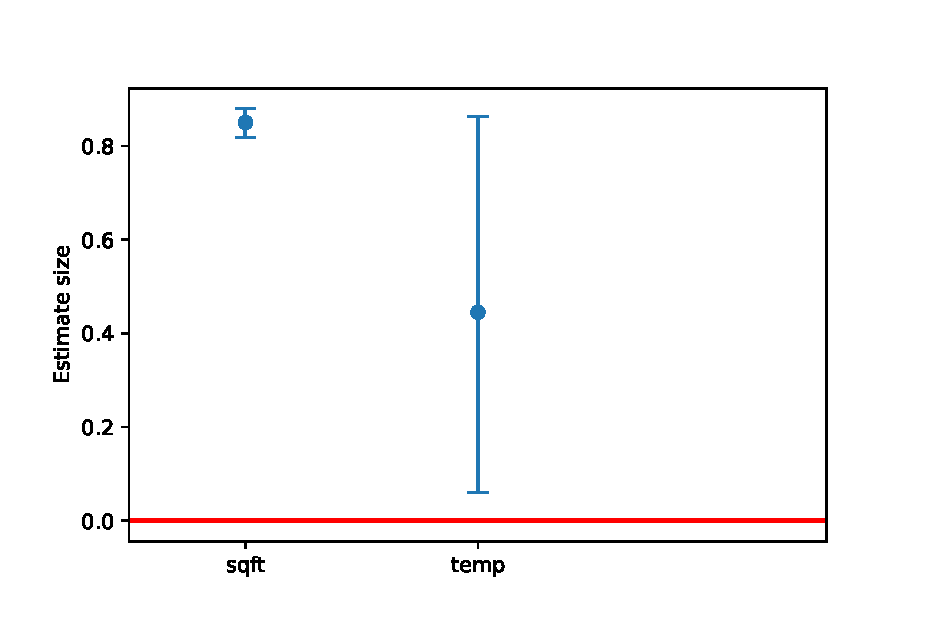
\includegraphics[scale = 0.7]{samplebars.eps}
    \caption{Average marginal effects estimates with 95\% confidence intervals bootstrapped using 1,000 replications.}
    \label{fig:samplebars}
\end{figure}

\end{document}
